% !TEX encoding = UTF-8
% !TEX program = pdflatex
% !TEX root = MEMOC.tex
% !TEX spellcheck = it-IT

\chapter{Il metodo del simplesso e la dualità}

Inizialmente abbiamo visto come le soluzioni di un problema di programmazione lineare intera si trovino sui vertici della regione ammissibile e come fosse possibile trovare una soluzione in modo grafico.

Con il metodo del simplesso vengono fatte delle considerazioni simili, però a livello algebrico, in modo che possano essere generalizzate a casi che utilizzano più di due variabili.

\section{Le basi del simplesso}

La struttura generale di un modello è:

\begin{align*}
	\min(\max)\: &f(x) \\
		\st &g_i(x) = b_i \\
			&g_i(x) \leq b_i \\
			&g_i(x) \geq b_i \\
			&x \in \mathbb{R}^n
\end{align*}

\noindent dove $x$ è un vettore colonna di $n$ variabili reali, $f$ è la funzione obiettivo, $g_i$ sono le funzioni che rappresentano i vincoli (sono tutte funzioni $\mathbb{R}^n \to \mathbb{R}$) e i vari $b_i$ sono valori reali.

La cosa chiave è che i valori \textbf{sono numeri reali} e i vincoli sono \textbf{funzioni lineari}.

Si ha quindi che una \textbf{soluzione ammissibile} $x \in \mathbb{R}^n$ è un vettore che soddisfa tutti i vincoli, mentre la \textbf{regione ammissibile} è data dall'insieme delle soluzioni ammissibili e la soluzione ottima è una particolare soluzione ammissibile che minimizza (o massimizza) la funzione obiettivo.

Il processo di risoluzione consiste quindi nel determinare se:

\begin{itemize}
	\item Il problema è non ammissibile.
	\item Il problema è illimitato.
	\item Il problema ha una soluzione ottima.
\end{itemize}

\noindent La regione ammissibile può essere rappresentata come un \textbf{poliedro}, un'intersezione di un numero finito di semi-spazi chiusi e iperpiani in $\mathbb{R}^n$.

Un problema può quindi essere modellato come:

$$
\min (\max) \{c^T x : x \in P\}
$$

\noindent dove $P$ è un poliedro in $\Rn$.

\begin{figure}[htbp]
	\centering
	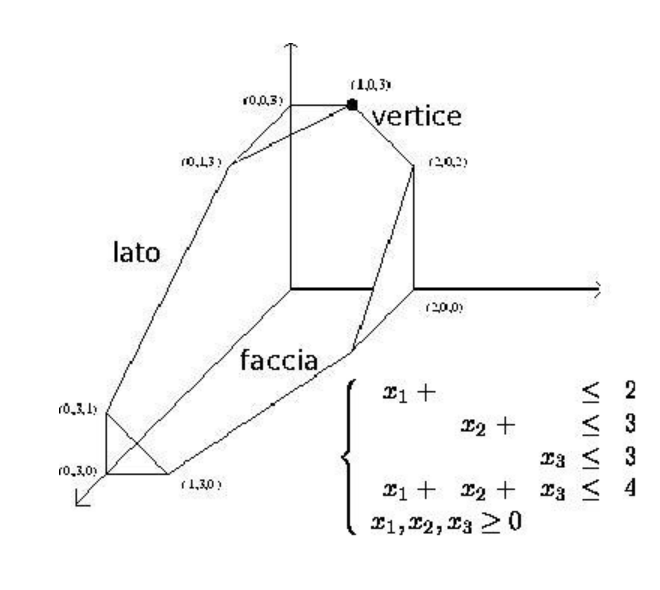
\includegraphics[width=0.6\textwidth]{images/l9-fig-1.png}
\end{figure}

\noindent Un \textbf{vertice} $v \in P$ è un vertice del poliedro $P$ se non è una \textbf{strict convex combination} di due punti distinti di $P$.

Un vertice $z \in \Rn$ è una \textbf{combinazione convessa} di due punti quando

$$
\exists \lambda \in [0,1] : z = \lambda x + (1-\lambda)y
$$

\noindent Viene detta \textbf{strict} se i valori 0 e 1 sono esclusi dall'intervallo.

Una \textbf{combinazione convessa} può essere fatta anche con più di due punti e può essere utilizzata per rappresentare una regione.
$z \in \Rn$ è una combinazione convessa di $x^1, x^2, \ldots, x^k$ se $\exists \lambda_1, \lambda_2, \ldots \lambda_k \geq 0$ tale che 

$$
\sum\limits_{i=1}^{k} \lambda_i = 1 \quad \text{e}\quad z = \sum\limits_{i=1}^{k} \lambda_ix^i
$$

\noindent Per il teorema di \textbf{Minkowski-Weyl}, la combinazione convessa di tutti i vertici di un poliedro permettono di rappresentare tutti i punti che appartengo al poliedro.

Quindi, per il \textbf{teorema del vertice ottimo}, se un problema LP ha può essere rappresentato da un poliedro $P$, allora esiste almeno una soluzione ottima e una di queste è su un vertice.

Questo è un risultato importante perché possiamo limitare la ricerca della soluzione ottima sui vertici di $P$ e non su tutto lo spazio.

\subsection{Rappresentazione algebrica dei vertici}

Considerando tutti i vincoli come delle uguaglianze abbiamo che i vertici del poliedro sono ottenuti intersecando tra loro le rette rappresentate dai vincoli (considerando il caso con due variabili).

Per trasformare i vincoli da disuguaglianze in uguaglianze è necessario aggiungere delle variabili di \textit{slack} che simulano il maggiore o minore.

Ad esempio:

	\begin{align*}
	3x_1 + 4x_2 &\leq 24 \\
	x_1 + 4x_2 &\leq 20 \\
	3x_1 + 2x_2 &\leq 18
	\end{align*}


\noindent diventa



	\begin{align*}
	3x_1 + 4x_2 +s_1&= 24 \\
	x_1 + 4x_2 +s_2&= 20 \\
	3x_1 + 2x_2 +s_3&= 18
	\end{align*}



Se si crea un sistema con queste nuove equazioni si ottengono due gradi di libertà, ovvero possiamo porre due variabili qualsiasi a zero per ottenere una soluzione unica.
Ad esempio se $s_1 = s_2=0$, otteniamo un sistema che può essere risolto e la cui soluzione rappresenta il vertice nel quale vengono imposti saturi il primo e secondo vincolo.

\subsection{Forma standard di un problema}

Per rendere l'approccio generico assumiamo che tutti i problemi sono scritti secondo la forma standard:

\begin{align*}
\min \: &c_1x_1+ c_2x_2 +\ldots + c_nx_n \\
\st &a_{i1}x_1 + a_{i2}x_2 +\ldots+a_{in}x_n = b_i \quad (i = 1 \ldots m) \\
&x_i \in \mathbb{R}_+ \quad (i = 1 \ldots n)
\end{align*}

\noindent Ovvero un problema in quale si minimizza sempre la funzione obiettivo, con tutte le variabili $\geq 0$ (per rendere semplice identificare le soluzioni non ammissibili), con tutti i vincoli che sono uguaglianze e con tutte le parti destre $b_i$ dei vincoli $\geq 0$.

Si può sempre trasformare un problema generico in forma standard.

\begin{itemize}
	\item Se il problema iniziale è una massimizzazione, basta passare alla minimizzazione e moltiplicare la funzione obiettivo per $-1$.
	\item Se ci sono delle variabili negative è possibile sostituirle con un'altra variabile che è positiva, es $x_+ = - x_\text{-}$.
	\item Se ci sono delle disuguaglianze è possibile aggiungere le variabili slack.
	\item Se un $b_i$ è negativo si può moltiplicare tutto il vincolo per $-1$. 
\end{itemize}

\section{Il metodo del simplesso}

\noindent Assumiamo che il problema sia modellato dal sistema $Ax = b$, $A \in \R^{m\times n}, \rho(A) = m, m <n$.
Definiamo come \textbf{base di $A$} una sotto-matrice quadrata $B \in \R^{m \times m }$ tale che abbia rango massimo, ottenuta prendendo $n$ colonne linearmente indipendenti della matrice $A$. 

Abbiamo quindi che $A = [B|N]$ con $det(B) \neq 0$ e $x = \begin{bmatrix}
x_B\\ 
x_F
\end{bmatrix}$ con $x_B \in \R^m$ e $x_F \in \R^{n-m}$.

Così facendo possiamo riscrivere il sistema come 

\begin{align}
Ax &= b \\
[B|F]\begin{bmatrix}
x_B\\ 
x_F
\end{bmatrix} &= b\\
B x_B + F x_F &= b
\end{align}

\noindent Posso quindi ricavare i valori di $x_B$, ovvero delle variabili presenti nella base con

$$
x_B = B^{-1}b - B^{-1}F x_F
$$

\noindent Ponendo le variabili $x$ fuori base ($x_F$) uguali a 0, otteniamo una \textbf{soluzione base}.
Il nome \textbf{base} deriva dal fatto che l'insieme dei vettori che compongono la base sono tutti linearmente indipendenti.

Quindi in una soluzione base abbiamo almeno $n-m$ variabili uguali a 0 (se ce ne sono di più la base diventa degenere).

Tornando al nostro problema di partenza abbiamo che una soluzione base diventa \textbf{ammissibile} quando soddisfa tutti i vincoli di partenza, ovvero

$$
x_B = B^{-1}b \geq 0
$$

\noindent Inoltre, per la proprietà di \textbf{corrispondenza tra vertici e soluzioni di base} si ha che se $x$ è una soluzione di base, allora
\begin{equation}
Ax = b \Leftrightarrow x \text{ è vertice di }P 
\end{equation} 
 
Per ottenere delle basi diverse, e quindi cercare un altro vertice, basta cambiare quali variabili sono fissate a 0.

Combinando ciò con il teorema del vertice ottimo si ottiene il \textbf{Teorema fondamentale delle programmazione lineare}, il quale asserisce che se esiste una soluzione ottima allora esiste anche una soluzione di base ammissibile e ottima.

Da qui nasce l'idea del metodo del simplesso, il quale parte da un problema posto in forma standard e da una soluzione ammissibile per trovare un vertice ottimo.

\subsection{I passi dell'algoritmo}

L'algoritmo del simplesso considera un problema in forma standard e necessita di una soluzione ammissibile di base di partenza.
L'algoritmo passa iterativamente da una soluzione ammissibile di base ad una adiacente che permetta di migliorare il valore corrente della funzione obiettivo fino al raggiungimento dell'ottimo.

\subsection{Passo -1: Passaggio alla forma standard}

Trasformo il problema nella forma

\begin{align*}
\min \:& z=c^Tx \\
\st& Ax=b \\
&x\geq 0
\end{align*}

\subsection{Passo 0: Base iniziale e tableau}

Fisso una base iniziale di partenza e riscrivono il problema in modo che:

\begin{itemize}
\item Nei vincoli, le variabili di base siano espresse solamente nei termini delle variabili fuori base.
\item La funzione obiettivo contenga solo variabili non di base
\end{itemize}

\noindent ovvero il problema diventa:

\begin{align*}
\min \: z=\: &c_{B}^T B^{-1}b + (c_{F}^T - c_{B}^T B^{-1}F)x_F \\
\st& Ix_B + B^{-1}Fx_F = B^{-1}b \\
&x\geq 0
\end{align*}

\noindent che può essere sintetizzato in 

\begin{align*}
\min \: z=\: &z_B + \overline{c}_{F}^Tx_F \\
\st& Ix_B + \overline{F}x_F = \overline{b} \\
&x\geq 0
\end{align*}

\noindent dove:

\begin{itemize}
\item $ \overline{b} =  B^{-1}b $ rappresenta il valore delle variabili di base nella soluzione corrente.
\item $ z_B =  c_{B}^T B^{-1}b$ è il valore corrente della funzione obiettivo.
\item $ \overline{F} = B^{-1}F $ sono le colonne delle variabili fuori base espresse nei termini della base corrente.
\item $ \overline{c}_{F}^T = c_{F}^T - c_{B}^T B^{-1}F$ sono i costi ridotti per le variabili fuori base.
\end{itemize}

Questa forma prende il nome di \textbf{forma tableau} o forma canonica.

\begin{table}[htbp]
\centering
\begin{tabular}{c|c|c|c|}
\cline{2-4}
$-z$ & $-z_B$           & $0$     & $\overline{c}_{F}^T$ \\ \cline{2-4} 
   & $\overline{b}$ & $Ix_B$ & $\overline{F}x_F$         \\ \cline{2-4} 
\end{tabular}
\end{table}

\begin{figure}[htbp]
	\centering
	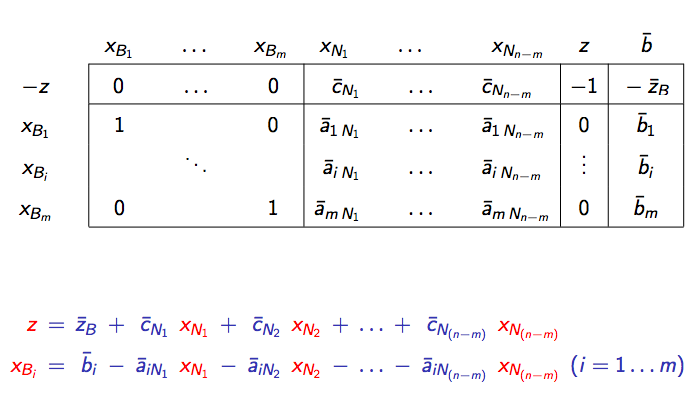
\includegraphics[width = .7\textwidth]{images/l9-fig-3.png}
	\caption{Il talbeau del simplesso}
\end{figure}

\subsection{Passo 1: Scelta della variabile da fare entrare in base}

L'operazione di cambio base permette di passare da una soluzione ammissibile di base ad una adiacente.

Considerando l'espressione della funzione obiettivo in termini di variabili fuori base, ovvero considerando la prima riga del tableau, abbiamo che:

\begin{align*}
z &= z_B + \overline{C}_{F}^Tx_F \\
&= z_B + \overline{C}_{F_1}^Tx_{F_1} + \ldots + \overline{C}_{F_n}^Tx_{F_n}
\end{align*}

Se entra in base una nuova variabile $x_{F_j}$, ovvero diventa diversa da 0, si ha che il nuovo valore della funzione obiettivo diventerà

$$
z = z_B + \overline{C}_{F_j}^Tx_{F_j}
$$

dove $\overline{C}_{F_j}$ rappresenta l'incremento marginale della funzione obiettivo all'aumentare di $x_{F_j}$ e viene detto costo ridotto. 

\subsection{Passo 2: Scelta della variabile uscente}

La nuova variabile che entra in base deve assumere il massimo valore possibile che non rende inammissibile la soluzione.
Pertanto viene assegnato alla variabile entrante $x_j$ il valore $\vartheta$ che preserva l'ammissibilità della soluzione, ovvero non rende le altre variabili negative.

Il valore $\vartheta$ viene scelto con la \textbf{regola del quoziente}

$$
\vartheta = \min\limits_{i | \overline{a}_{ij} > 0} \bigg\{ \frac{\overline{b}_i}{\overline{a}_{ij}} \bigg\}
$$

dove $\overline{a}_{ij}$ è il coefficiente di $x_j$ nel vincolo $i$.

La variabile uscente è quindi quella che corrisponde al minimo quoziente, ovvero a quella che viene azzerata ponendo $x_j = \vartheta$.

Da notare che se tutti gli $\overline{a}_{ij}$ sono $\leq 0$, il problema è illimitato, perché la variabile $x_j$ può entrare in base con un valore qualsiasi, migliorando sempre la funzione obiettivo.

\subsection{Passo 3: Cambio di base} 

Se $x_j$ è la variabile selezionata per entrare in base e $x_k$ è la variabile uscente è necessario effettuare un'operazione di pivot della matrice in modo che la colonna corrispondente a $x_j$ diventi della forma $ \begin{bmatrix}
0\\ 
e_k
\end{bmatrix} $ dove $e_j$ è un vettore di 0 con l'elemento di indice $j = 1$.

\subsection{Passo 4: Condizione di terminazione}

Il metodo del simplesso continua fino a che non ci sono più costi ridotti negativi e pertanto la soluzione di base è anche ottima.

Bisogna però stare attenti a non visitare sempre la stessa sequenza di vertici. Per evitare ciò è possibile scegliere di far entrare in base sempre la variabile di indice minimo tra tutte quelle che hanno costi ridotti negativi.



\subsection{Algoritmo del simplesso nel dettaglio}

\begin{enumerate}
	\item Trasforma il PL in forma standard e trova una base iniziale feasible $B$. La base può essere trovata risolvendo un problema artificiale.
	\item Ripeti finché non trovi una soluzione ottima o non ti accorgi che il problema è illimitato:
	\begin{itemize}
		\item Poni il problema in forma canonica rispetto la base $B$
		\begin{align*}
		z &= \overline{z}_B + \overline{c}_{F_1} x_{F_1} 
		+ \overline{c}_{F_2} x_{F_2} + \ldots + \overline{c}_{F_{n-m}} x_{F_{n-m}} \\
		x_{B_i} &= \overline{b}_i - \overline{a}_{iF_1} x_{F_1} - \overline{a}_{iF_2} x_{F_2} - \ldots - \overline{a}_{iF_{n-m}} x_{F_{n-m}} \qquad \forall \: i \in [1 \ldots m]
		\end{align*}
		\item Se $\overleftarrow{c}_j \geq 0 \forall \ j$, la base $B$ è ottima. Fermati.
		\item Se $\exists h : \overline{c}_h < 0 , \overline{a}_{ih}\leq 0 \ \forall i$, il problema è illimitato. Fermati.
		\item Scegli una variabile $x_h$ da portare in base tra tutte quelle con costi ridotti negativi.
		\item Trova la variabile $x_{B_t}$ con $ t = \arg \min_{i = 1 \ldots m} \bigg\{ \frac{\overline{b}_i}{\overline{a}_{ih}}  : \overline{a}_{ih} > 0 \bigg\}$
		\item $B \leftarrow B \oplus A_h \ominus A_{B_t}$, ovvero effettua il cambio di base.
	\end{itemize}
\end{enumerate}

Da notare che tutti i vari passaggi possono essere replicati utilizzando i calcoli matriciali al posto del tableau del simplesso.


\subsection{Metodo delle due fasi}

Questo metodo permette di trovare una soluzione ammissibile di partenza per il metodo del simplesso.

Dato un problema in forma standard

\begin{align*}
\min \:& z=c^Tx \\
\st& Ax=b \\
&x\geq 0
\end{align*}

\noindent viene creato un problema artificiale, aggiungendo al problema di partenza un nuovo vettore di variabili $y \in \R^{m}$ e cambiando la funzione obiettivo:

\begin{align*}
w^* = \min \:& w= I^Ty = y_1 + y_2 + \ldots + y_m \\
\st& Ax + Iy=b \\
&x, y\geq 0
\end{align*}

Per come è formulato questo problema ho già che $Iy$ è una base ammissibile ma non ancora espressa in forma canonica.
Inoltre, questo problema è sempre ammissibile, perché la soluzione $x = 0, y=b$ è ammissibile ed inoltre non è mai illimitato perché la funzione obiettivo è la minimizzazione di una sommatoria con termini tutti maggiori di 0, pertanto l'ottimo è 0.

Una volta messo in forma canonica il problema artificiale, posso risolverlo utilizzando il simplesso ottenendo un valore ottimo $w*$, che può essere:

\begin{itemize}
\item $w^* > 0$: il problema originale non è ammissibile e quindi non ha senso passare alla fase 2.
\item $w^* = 0$: in questo caso tutte le variabili artificiali sono necessariamente nulle e quindi possono essere tolte dai vincoli, rendendoli comunque soddisfatti, pertanto il problema di partenza è ammissibile. Se tutte le $y$ sono fuori base, allora il tableau finale può essere usato come tableau di partenza per il simplesso sul problema originale, altrimenti è necessario effettuare un cambio di base in modo da togliere dalla base tutte le $y$.


\end{itemize}
















